% 原书 p.92–p.98（PDF p.100–p.106）
% 第 4 章 4.3 节：邻域定理

% >>> p100
\section{邻域定理（Neighborhood Theorems）}

\begin{keytakeaways}
\begin{itemize}
  \item 几何图像：局部模型（Darboux 模型、管状邻域模型、Weinstein 邻域模型）之所以「处处
        相同」，是因为 Moser 论证能把在小邻域上彼此相等的两个形式用微分同胚拉回。
  \item 数学工具：指数映射与法丛、近复结构 $J$ 及其度量 $g_J$、同构
        $\beta\colon JTL\to NL\to T^*L$。
  \item 本节结论：辛与切触的 Darboux 定理（定理 4.3.1、4.3.2）、Weinstein 邻域定理
        （定理 4.3.3）、Legendre 邻域定理（练习 4.3.1），以及 $\Symp(M,\omega)$ 在
        恒等映射附近的 $C^1$-邻域与闭 $1$-形式空间零点的对应（例 4.3.2）。
\end{itemize}
\end{keytakeaways}

Moser 论证使我们能够导出许多有用的「邻域平凡性」结果：在这些邻域中工作等价于在标准模型
中工作。让我们从下面的引理开始。

\begin{wlem}{4.3.1}
  设 $M$ 是光滑流形（不必紧），$Q\subset M$ 是紧子流形。假设 $\omega_0,\omega_1$ 是
  $M$ 上的辛形式，且对任意 $q\in Q$ 都有 $\omega_0|_{T_qM}=\omega_1|_{T_qM}$。则存在
  $Q$ 在 $M$ 中的开邻域 $U_0,U_1$ 以及微分同胚 $\varphi\colon U_0\to U_1$，使得
  $\varphi^*\omega_1=\omega_0$ 且 $\varphi|_Q=\mathbf 1$。这个关系可用下图表示，
  其中 $i$ 是嵌入映射。
\end{wlem}

\begin{figure}[htbp]
  \centering
  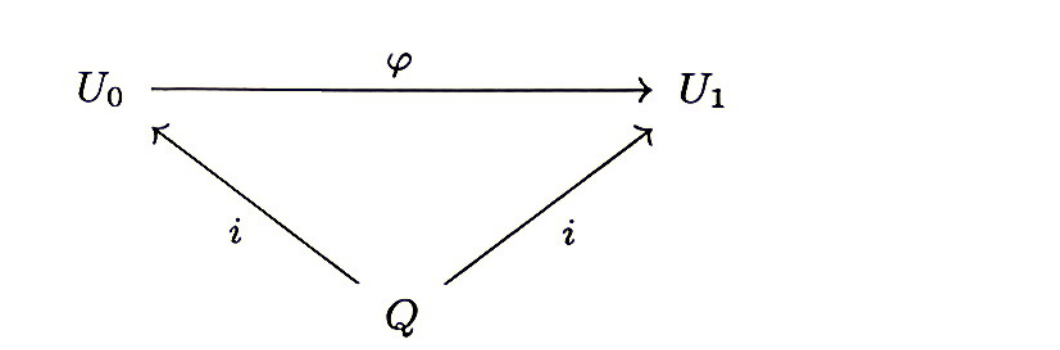
\includegraphics[width=0.55\linewidth]{figures/fig_p100_1.png}
  \caption*{原书 p.92 示意图（无编号）：引理 4.3.1 中的交换关系，$i$ 为嵌入映射
  （PDF p.100）}
\end{figure}
% [Tutor Note: 术语/结构——引理断言的是「局部相对版本」：条件只在 Q 上的点处要求两个
% 2-形式相等（ω_0|_{T_qM} = ω_1|_{T_qM} 指在 q 点对任意切向量相等，而不只是沿 T_qQ
% 相等），结论只保证在 Q 的某个小邻域内存在把 ω_1 拉回 ω_0 的微分同胚，并且该微分
% 同胚在 Q 上为恒等。注意 Q 紧、M 不必紧；证明放在本章末（p.100），思路是先做「线性形变
% ω_t = (1−t)ω_0 + tω_1」，再用管状邻域把 Q 的邻域拉直，最后用 Moser 论证。]

理解上述这类精细结果的一种方式是：先用它（而不急于证明它）。著名的 Darboux 定理可以
很容易地由它推得。

% >>> p101
\begin{wthm}{4.3.1}（Darboux 定理，前面定理 1.2.1 中已提及）
  每个辛流形 $(M^{2n},\omega)$ 都局部辛同胚于 $(\R^{2n},\omega_{\mathrm{std}})$ 中
  $0$ 的一个开邻域。
\end{wthm}

\begin{figure}[htbp]
  \centering
  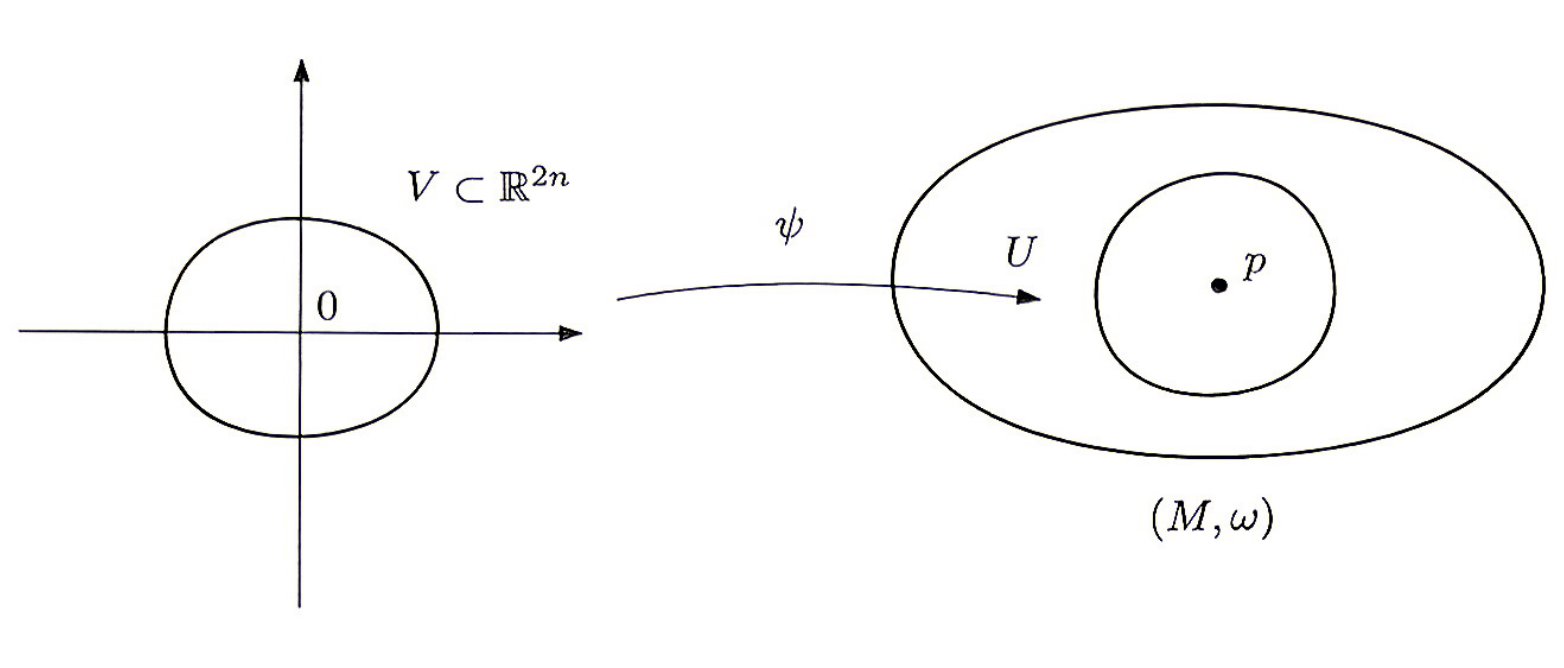
\includegraphics[width=0.85\linewidth]{figures/fig_p101_1.png}
  \caption*{图 4.1\quad Darboux 定理（原书 p.93, Figure 4.1；PDF p.101）}
\end{figure}

\begin{wproof}
  由于 $M$ 是流形，存在 $p\in M$ 的邻域 $U$、$0\in\R^{2n}$ 的邻域 $V$，以及
  微分同胚 $\psi\colon V\to U$（见图 4.1）。

  于是在 $V$ 上得到辛结构 $\psi^*(\omega|_U)$。注意在这个邻域 $V$ 中，两个辛结构
  $\psi^*(\omega|_U)$ 与 $\omega_{\mathrm{std}}|_V$ 未必重合。但在 $0\in\R^{2n}$ 处，
  $\psi^*(\omega|_U)$ 与 $\omega_{\mathrm{std}}|_V$ 相差一个线性辛同构（见图 4.2）。
  取 $A\in\Sp(2n)$ 使得 $A\cdot\psi^*(\omega|_U)|_0=(\omega_{\mathrm{std}}|_V)|_0$。
  于是在 $V$ 上定义两个辛结构如下：
  \begin{equation*}
    \omega_0:=A\cdot\psi^*(\omega|_U)\quad\text{和}\quad
    \omega_1:=\omega_{\mathrm{std}}|_V.
  \end{equation*}

  \begin{figure}[htbp]
    \centering
    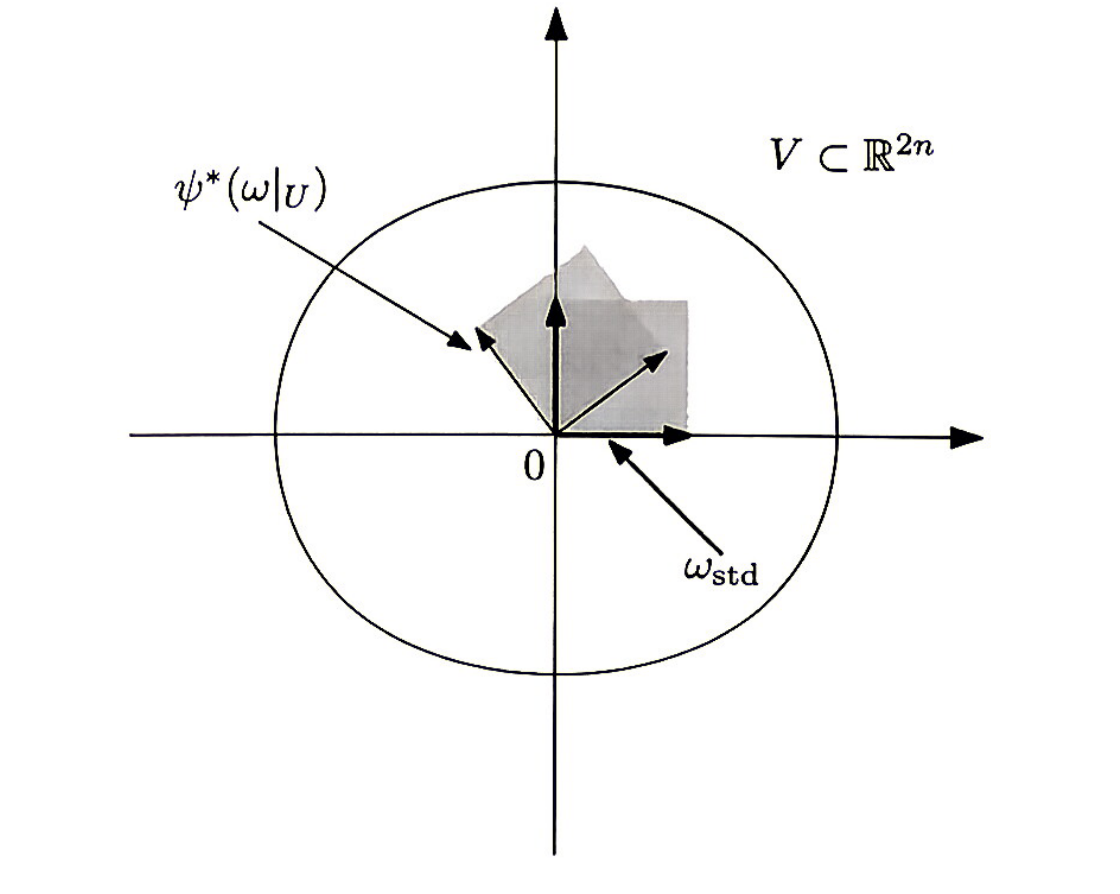
\includegraphics[width=0.5\linewidth]{figures/fig_p101_2.png}
    \caption*{图 4.2\quad $V$ 上的辛结构（原书 p.93, Figure 4.2；PDF p.101）}
  \end{figure}

  它们满足引理 4.3.1 中的条件（其中 $Q=\{0\}$），于是存在 $0\in\R^{2n}$ 在 $V$ 中的
  邻域 $U_0,U_1$ 以及微分同胚 $\varphi\colon U_0\to U_1$，使得
  \begin{equation*}
    \varphi^*\bigl((\omega_{\mathrm{std}}|_V)|_{U_1}\bigr)
    =(A\cdot\psi^*(\omega|_U))|_{U_0}\quad\text{且}\quad\varphi|_0=\mathbf 1.
  \end{equation*}
  这等价于
  $\omega_{\mathrm{std}}|_{U_1}
  =(\varphi^{-1})^*\bigl(A\cdot\psi^*(\omega|_U)\bigr)|_{U_0}$。
  于是得到所需的辛同胚。
\end{wproof}
% [Tutor Note: 易错预警——证明的关键是「先在一点对齐」：任意两个辛形式在一点只相差一个
% 线性同构（线性辛群 Sp(2n) 在非退化 2-形式上可迁），故可取 A ∈ Sp(2n) 使 A·ψ^*(ω|_U)|_0
% 与 (ω_std|_V)|_0 在 0 点相等；然后对 Q = {0} 用引理 4.3.1。注意 A 作用在形式上、而
% 线性辛同构作用在切空间上，不同教材对 A·ω 的约定（用 A 还是 A^{-1}）不同，核对时以
% 「A·ψ^*(ω|_U)|_0 = (ω_std|_V)|_0 在 0 点成立」为准。]

对于切触流形，我们有 Darboux 定理的类似版本。

% >>> p102
\begin{wthm}{4.3.2}（切触几何中的 Darboux 定理）
  对任意切触流形 $(M^{2n+1},\xi=\ker\alpha)$，它局部严格切触同胚于
  $(\R^{2n+1},\xi_{\mathrm{std}}=\ker\alpha_{\mathrm{std}})$ 的一个开邻域。特别地，
  局部地经由严格切触同胚，切触 $1$-形式 $\alpha$ 可等同于
  $\alpha_{\mathrm{std}}=\dd z-\sum_{i=1}^n y_i\,\dd x_i$。
\end{wthm}

\begin{wproof}
  对任意 $p\in(M,\xi=\ker\alpha)$，如图 4.3，设 $\psi$ 是从 $0\in\R^{2n+1}$ 的邻域
  $V\subset\R^{2n+1}$ 到 $p\in M$ 的邻域 $U$ 的微分同胚。在 $0\in\R^{2n+1}$ 处，
  $V$ 中两个切触 $1$-形式 $\psi^*\alpha$ 与 $\alpha_{\mathrm{std}}$ 相差一个矩阵
  $A\in M_{(2n+1)\times(2n+1)}(\R)$，即
  \begin{equation}\tag{4.15}
    A\cdot\psi^*\alpha|_0=\alpha_{\mathrm{std}}|_0.
  \end{equation}

  \begin{figure}[htbp]
    \centering
    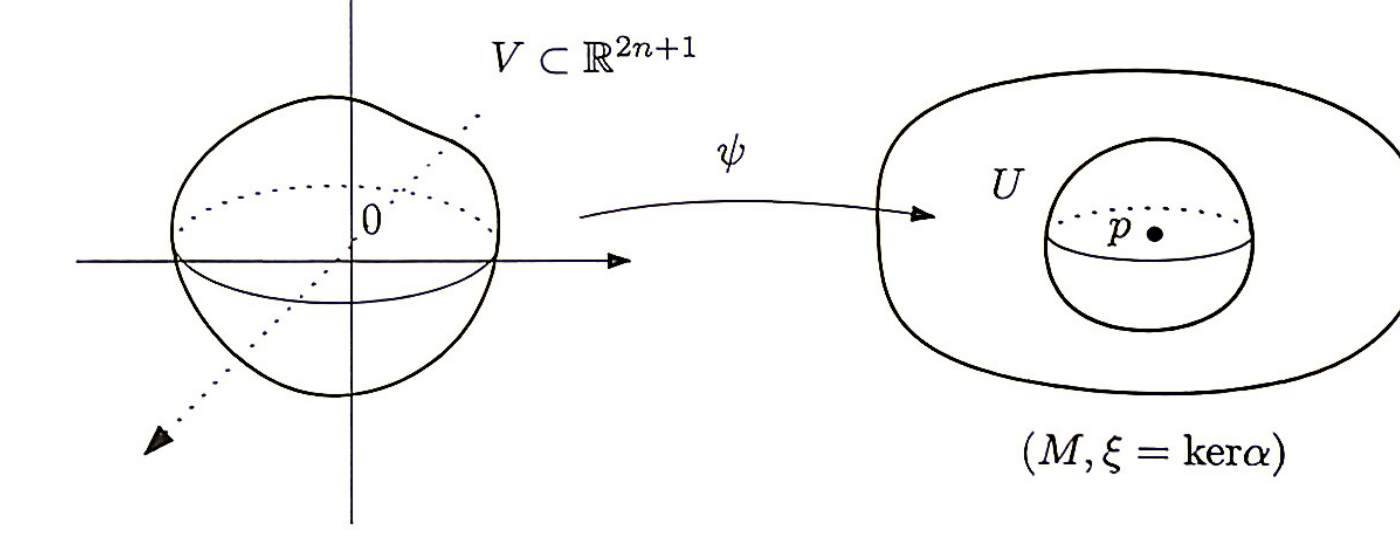
\includegraphics[width=0.8\linewidth]{figures/fig_p102_1.png}
    \caption*{图 4.3\quad 切触几何中的 Darboux 定理（原书 p.94, Figure 4.3；PDF p.102）}
  \end{figure}

  考虑 $A\cdot\psi^*\alpha$ 与 $\alpha_{\mathrm{std}}$ 在 $V$ 上的线性组合
  \begin{equation}\tag{4.16}
    \alpha_t:=(1-t)\alpha_{\mathrm{std}}+tA\cdot\psi^*\alpha.
  \end{equation}
  特别地，在 $0\in\R^{2n+1}$ 处有 $\alpha_t|_0=\alpha_{\mathrm{std}}|_0$ 以及
  $\dd\alpha_t|_0=\dd\alpha_{\mathrm{std}}|_0$。由于
  $\alpha_{\mathrm{std}}\wedge(\dd\alpha_{\mathrm{std}})^n\neq0$ 在
  $0\in\R^{2n+1}$ 处成立，在 $V$ 的某个小邻域 $U\subset V$ 中，
  $\alpha_t\wedge(\dd\alpha_t)^n\neq0$ 对一切 $t\in[0,1]$ 成立。换言之，由上述线性
  组合定义的 $\{\alpha_t\}_{t\in[0,1]}$ 确实是 $U$ 上的一族光滑切触 $1$-形式。

  为了得到 $U$ 中的光滑切触同痕 $\{\varphi_t\}_{t\in[0,1]}$ 使得
  $\varphi_t^*\alpha_t=\alpha_0$，我们将重新回到 Moser 论证（更具体地说，是 4.1 节
  定理 4.1.2 的证明）。对 $\varphi_t^*\alpha_t=\alpha_0$ 两边求导，得
  \begin{equation*}
    \varphi_t^*\Bigl(\frac{\dd\alpha_t}{\dd t}
    +\iota_{X_t}\dd\alpha_t+\dd(\alpha_t(X_t))\Bigr)=0.
  \end{equation*}
\end{wproof}

% >>> p103
所以我们要求一个向量场 $X_t$ 满足
\begin{equation}\tag{4.17}
  \frac{\dd\alpha_t}{\dd t}+\iota_{X_t}\dd\alpha_t+\dd(\alpha_t(X_t))=0.
\end{equation}
由 $TM$ 的分解，可写 $X_t=a(t)R_{\alpha_t}+Y_t$，其中 $a(t)$ 是系数函数，
$Y_t\in\xi_t=\ker\alpha_t$。于是 (4.17) 等价于
\begin{equation}\tag{4.18}
  \frac{\dd\alpha_t}{\dd t}+\iota_{Y_t}\dd\alpha_t+\dd a(t)=0.
\end{equation}
在 (4.18) 两边代入 $R_{\alpha_t}$，得
\begin{equation}\tag{4.19}
  \frac{\dd\alpha_t}{\dd t}(R_{\alpha_t})+\dd a(t)(R_{\alpha_t})=0.
\end{equation}
观察可知，上式中的 $a(t)$ 有局部解（但未必有整体解）。一旦由 (4.19)（局部地）解出
$a(t)$，便可由 (4.18) 解出 $Y_t$。积分 $X_t$ 即得所需的同痕 $\varphi_t$。再把时间
$1$ 映射 $\varphi_1$ 与 $\psi$、以及 (4.15) 中的矩阵 $A$ 作适当复合，便得到所需的
切触同胚。
% [Tutor Note: 含糊点拨——(4.19) 是关于 a(t) 的一阶线性方程，沿 R_{α_t} 的轨道看它就是
% 一个常微分方程：da(t)(R_{α_t}) = −(dα_t/dt)(R_{α_t})。它在每条 Reeb 轨道上可（局部）
% 解出 a，但整体解可能因闭轨道上的周期条件而不存在；好在 Darboux 定理只要求局部结论，
% 故取足够小的 U 即可。这与定理 4.1.2 的差别在于：那里已给出全局的 α_t，因而可用
% 全局 Moser 论证；这里 α_t 只在小邻域内有定义。]

\begin{wrem}{4.3.1}
  注意，对 (4.16) 中的 $\alpha_t$，$\{\xi_t=\ker\alpha_t\}_{t\in[0,1]}$ 给出（局部的）
  一族切触结构。因此，若把定理 4.3.2 的要求减弱为「局部切触同胚于
  $(\R^{2n+1},\xi_{\mathrm{std}})$」（而不是经由\textbf{严格}切触同胚），则无需像
  定理 4.3.2 的后半部分那样重新回到 Moser 论证，直接由定理 4.1.2 即可完成证明。
\end{wrem}
% [Tutor Note: 术语依据——「严格切触同胚」指保持切触 1-形式（ψ^*α_std = α）的切触同胚；
% 若只要求保持切触结构（ψ_*ξ = ξ），则允许相差共形因子 e^f。定理 4.3.2 要求的是前者，
% 故不能直接用 Gray 定理（定理 4.1.2），必须再解一次 Moser 方程；注 4.3.1 说的正是这个
% 差别。]

下一个例子取自 [2] 第 2.1 节末的例子，由 H. Gluck 提供。它说明有时可以用显式的方式
得到定理 4.3.2 所承诺的切触同胚。

\begin{wexam}{4.3.1}
  考虑 $(\R^3,\xi=\ker\alpha)$，其中 $\alpha=\dd z+x\,\dd y-y\,\dd x$
  （$\neq\alpha_{\mathrm{std}}$）是切触 $1$-形式。我们可以找到一个整体定义的微分同胚
  $\varphi\colon\R^3\to\R^3$，使得 $\varphi^*\alpha=\alpha_{\mathrm{std}}$。事实上，
  在坐标 $(x,y,z)\in\R^3$ 中，$\varphi$ 可如下构造：
  \begin{equation}\tag{4.20}
    \varphi\colon(x,y,z)\mapsto\Bigl(\frac x2,\,y,\,z-\frac{xy}2\Bigr).
  \end{equation}
  我们很容易验证
  \begin{equation*}
    \begin{aligned}
      \varphi^*\alpha
      &=\dd\Bigl(z-\frac{xy}2\Bigr)+\frac x2\,\dd y-\frac y2\,\dd x\\
      &=\dd z-\frac12x\,\dd y-\frac12y\,\dd x+\frac12x\,\dd y-\frac12y\,\dd x\\
      &=\dd z-y\,\dd x=\alpha_{\mathrm{std}}.
    \end{aligned}
  \end{equation*}
  % [Tutor Note: 易错预警——第二行展开时注意 d(z−xy/2) = dz − (1/2)x dy − (1/2)y dx，
  % 而 φ^*x·dy 一项给出 (x/2)dy、φ^*(−y dx) 给出 −(y/2)dx（因为 φ^*x = x/2，
  % φ^*y = y，φ^*z = z−xy/2）；符号核对以最终得到 α_std = dz − y dx 为准。]

  下面我们将看到，如何按照定理 4.3.2 的证明，用 Moser 论证得到这个 $\varphi$。在
  $0\in\R^3$ 处，$\alpha|_0=\alpha_{\mathrm{std}}|_0=\dd z$，故 (4.15) 中的过渡矩阵 $A$

% >>> p104
  将取为恒等矩阵。然后按 (4.16) 考虑线性组合
  \begin{equation*}
    \begin{aligned}
      \alpha_t&=(1-t)\alpha_{\mathrm{std}}+t\alpha\\
      &=\dd z-(1-t)y\,\dd x+tx\,\dd y-ty\,\dd x\\
      &=\dd z-y\,\dd x+tx\,\dd y.
    \end{aligned}
  \end{equation*}
  对任意 $t\in[0,1]$，$1$-形式 $\alpha_t$ 始终是切触 $1$-形式，因为
  $\alpha_t\wedge\dd\alpha_t=(1+t)\,\dd x\wedge\dd y\wedge\dd z$。其次，设
  $X_t=f(t)R_{\alpha_t}+Y_t$，其中 $f(t)$ 是系数函数，$Y_t\in\xi_t=\ker\alpha_t$。
  注意此时对 (4.19) 中的第一项，有
  \begin{equation*}
    \frac{\dd\alpha_t}{\dd t}(R_{\alpha_t})
    =(x\,\dd y)\Bigl(\frac{\partial}{\partial z}\Bigr)=0.
  \end{equation*}
  于是可以放心地取 $f(t)=0$，从而 $X_t\in\xi_t$。结合 (4.18)，$X_t$ 可由如下方程组解出：
  \begin{equation*}
    \begin{cases}
      \dfrac{\dd\alpha_t}{\dd t}+\iota_{X_t}\dd\alpha_t=0\\[2pt]
      \alpha_t(X_t)=0
    \end{cases}.
  \end{equation*}
  在坐标 $(x,y,z)\in\R^3$ 中，上式等价于
  \begin{equation}\tag{4.21}
    \begin{cases}
      x\,\dd y+(1+t)\,\dd x\wedge\dd y\,(X_t,\cdot)=0\\[2pt]
      (\dd z-y\,\dd x+tx\,\dd y)(X_t)=0
    \end{cases}.
  \end{equation}
  设 $X_t=a(t)\partial_z+b(t)\partial_x+c(t)\partial_y$，其中 $a(t),b(t),c(t)$ 是系数
  函数，则
  \begin{equation*}
    x\,\dd y+(1+t)b(t)\,\dd y-(1+t)c(t)\,\dd x=0,
  \end{equation*}
  这蕴含
  \begin{equation*}
    c(t)=0\quad\text{和}\quad b(t)=-\frac{x}{1+t}.
  \end{equation*}
  代回 (4.21) 的第二个方程，得 $a(t)=-\dfrac{xy}{1+t}$。因此 $X_t$ 可写为
  \begin{equation}\tag{4.22}
    X_t=-\frac{xy}{1+t}\frac{\partial}{\partial z}-\frac{x}{1+t}\frac{\partial}{\partial x}.
  \end{equation}
  下面求解 (4.22) 中 $X_t$ 的流 $\varphi_t\colon\R^3\to\R^3$。按定义它满足
  \begin{equation}\tag{4.23}
    \frac{\dd}{\dd t}\varphi_t(x,y,z)=X_t\circ\varphi_t(x,y,z).
  \end{equation}
  把 $\varphi$ 写成坐标形式 $\varphi_t(x,y,z)=(u(t),v(t),w(t))$，则 (4.23) 可转化为
  \begin{equation*}
    \frac{\partial u}{\partial t}=-\frac{u}{1+t},\qquad
    \frac{\partial v}{\partial t}=0,\qquad
    \frac{\partial w}{\partial t}=-\frac{uv}{1+t},
  \end{equation*}

% >>> p105
  再结合初值条件 $(u(0),v(0),w(0))=(x,y,z)$。容易解出
  \begin{equation*}
    \begin{cases}
      u(x,y,z,t)=\dfrac{x}{1+t}\\[4pt]
      v(x,y,z,t)=y\\[4pt]
      w(x,y,z,t)=z-\dfrac{xyt}{1+t}
    \end{cases}
  \end{equation*}
  最后，时间 $1$ 映射为 $\varphi=\varphi_1(x,y,z)=\bigl(\tfrac x2,\,y,\,z-\tfrac{xy}2\bigr)$，
  与 (4.20) 一致。\hfill$//$
\end{wexam}
% [Tutor Note: 含糊点拨——「容易解出」的实质是三个解耦的初值问题：u' = −u/(1+t) 给出
% u = x/(1+t)（积分因子 1+t）；v 为常数；再把 u 代入 w' = −uv/(1+t) = −xy/(1+t)^2，
% 积分得 w = z − xyt/(1+t)（用 ∫_0^t ds/(1+s)^2 = t/(1+t)）。注意初值取在 t = 0 时
% 为 (x,y,z)，这正是「时间 0 映射为恒等」的要求。]

下一个结果是定理 4.3.1 的相对版本。这里「相对」是指：命题涉及辛流形的子流形。当子流形是
拉格朗日子流形时，该结果通常称为 \textbf{Weinstein 邻域定理}（前面定理 1.2.2 中已提及）。

\begin{wthm}{4.3.3}（Weinstein 邻域定理 [242]）
  设 $(M,\omega)$ 是辛流形，$L\subset M$ 是紧拉格朗日子流形。则存在 $L$ 在 $M$ 中的
  邻域 $V$、零截面 $0_L\subset T^*L$ 的邻域 $U$，以及微分同胚 $\varphi\colon U\to V$，
  使得 $\varphi^*(\omega|_V)=\omega_{\mathrm{can}}|_V$ 且 $\varphi|_L=\mathbf 1$。
\end{wthm}
% [Tutor Note: 原文疑误——此处 ω_can|_V 应为 ω_can|_U：φ 的定义域是 U ⊂ T^*L，
% 而 ω_can 是 T^*L 上的典范辛形式，故 φ^*(ω|_V) 与 ω_can|_U 才是同一个开集上的形式；
% 原书写作 ω_can|_V 系下标笔误。译文按原文照译，详见 qsg/notes/review_ch04.md。]

在给出定理 4.3.3 的证明之前，让我们回忆微分拓扑中下面这个邻域定理（它与辛结构无关）。

\begin{wthm}{4.3.4}（管状邻域定理）
  设 $M$ 是光滑流形，$L\subset M$ 是光滑子流形。则存在法丛 $NL$ 中零截面 $0_L$ 的邻域
  $U$ 与 $L$ 在 $M$ 中的邻域 $V$ 之间的微分同胚 $\psi$（见图 4.4）。
\end{wthm}

\begin{figure}[htbp]
  \centering
  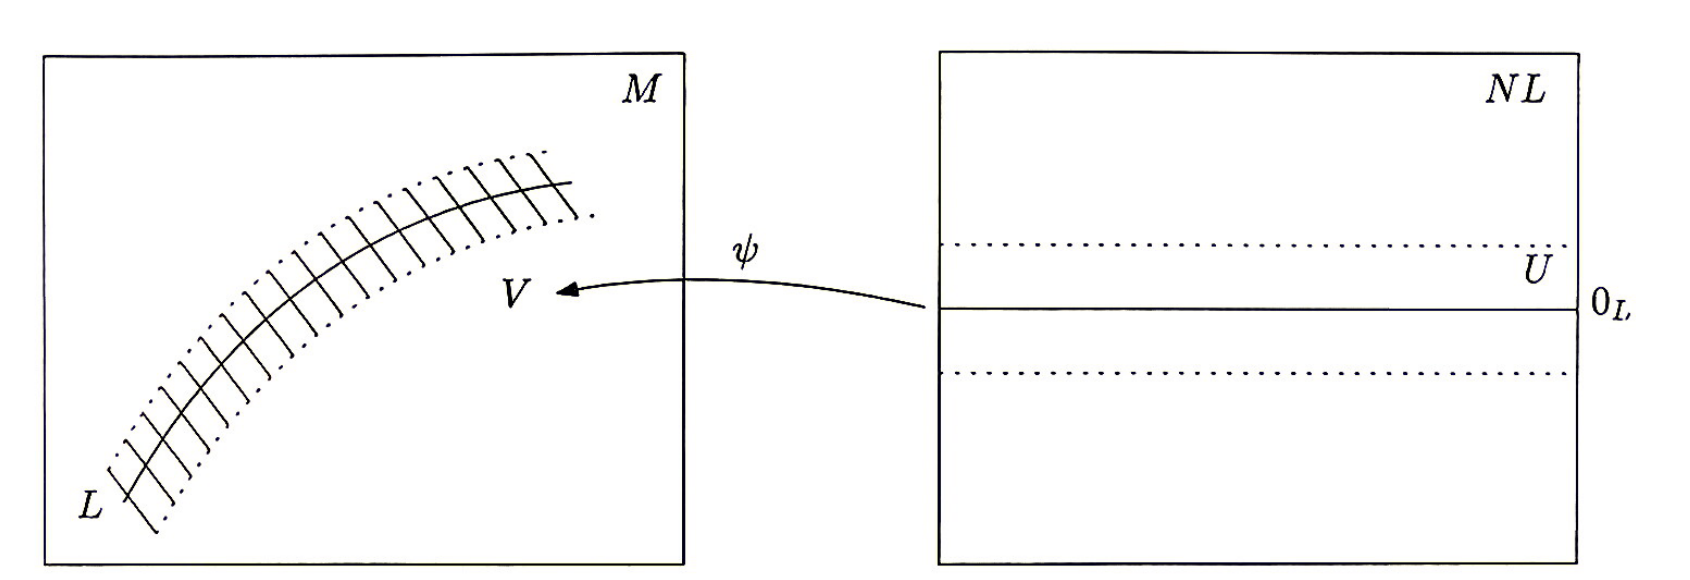
\includegraphics[width=0.85\linewidth]{figures/fig_p105_1.png}
  \caption*{图 4.4\quad 管状邻域定理（原书 p.97, Figure 4.4；PDF p.105）}
\end{figure}

定理 4.3.4 可通过直接应用 $M$ 上的指数映射 $\exp$ 来证明。其证明的标准参考文献是
[145] 中的定理 6.24、[102] 第 2 章（第 3 节）的练习 16。

作为证明定理 4.3.3 的另一项准备，回忆：对拉格朗日子流形 $L\subset M$，由命题 1.6.1
有同构 $NL\simeq T^*L$，其中 $NL$

% >>> p106
表示 $L$ 的法丛。结合定理 4.3.4，存在从 $T^*L$ 中 $0_L$ 的邻域 $U$ 到 $M$ 中 $L$ 的
邻域 $V$ 的微分同胚 $\psi$。与定理 4.3.1 中的论证类似，特别地，为了使用引理 4.3.1，
我们想说明 $\psi^*(\omega|_V)$ 的某个修正与 $L$ 上的 $\omega_{\mathrm{can}}$ 重合。

为此，我们在 $M$ 上选取一个与 $\omega$ 相容的近复结构 $J$。于是有下面几条观察：

\begin{enumerate}[label=(\roman*)]
  \item 正如 (1.8) 中提到的，$g_J(\cdot,\cdot)=\omega(\cdot,J\cdot)$ 是一个度量。
  \item 丛 $JTL$（在 $L$ 上），作为 $TL$ 在映射 $J$ 下的像，是 $TM$ 的拉格朗日子空间，
        因为对任意 $v,w\in TL$ 有 $\omega(Jv,Jw)=\omega(v,w)=0$。
  \item 在度量 $g_J$ 下，丛 $TL$ 与 $JTL$ 正交。具体地说，由上面 (i)，
\begin{equation*}
  g_J(v,Jw)=\omega(v,-w)=-\omega(v,w)=0
\end{equation*}
        对任意 $v,w\in TL$ 成立。
\end{enumerate}

$TL$、$JTL$ 与 $TM$ 之间的关系如图 4.5 所示。

\begin{figure}[htbp]
  \centering
  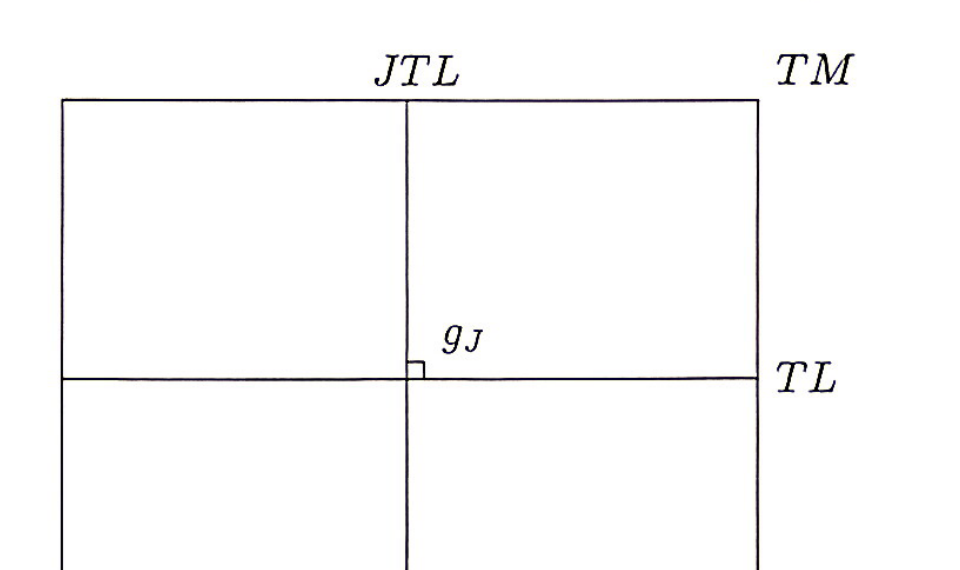
\includegraphics[width=0.45\linewidth]{figures/fig_p106_1.png}
  \caption*{图 4.5\quad $JTL$ 与 $TL$ 关于度量 $g_J$ 正交（原书 p.98, Figure 4.5；
  PDF p.106）}
\end{figure}
% [Tutor Note: 易错预警——(ii) 中 ω(Jv,Jw) = ω(v,w) 用的是 J 与 ω 相容（ω-compatible），
% 即 ω(J·,J·) = ω(·,·) 且 g_J 正定；(iii) 中 g_J(v,Jw) = ω(v,J(Jw)) = ω(v,−w) 用到了
% J^2 = −1。注意 (iii) 的「正交」是关于对称度量 g_J，而不是关于 ω（关于 ω，TL 是
% 拉格朗日子空间，与其自身正交，但与 JTL 的 ω-配对一般不为零）。]

观察 (i)、(ii)、(iii) 蕴含 $JTL\simeq NL$。事实上，对任意 $v\in JTL$，映射
$v\mapsto[v]\in NL=T_LM/TL$ 是单射（因为由上面的 (iii)，
$TL\cap JTL=\{0\}$）。此外，关于度量 $g_J$，(ii) 与 (iii) 蕴含
$T_pM=T_pL\oplus JT_pL$。于是由维数理由，映射 $v\mapsto[v]$ 也是满射，从而是同构。
因此，结合命题 1.6.1 的证明中所确认的同构 $NL\to T^*L$，我们得到如下复合
\begin{equation}\tag{4.24}
  \beta\colon JTL\to NL\to T^*L,\qquad
  v\mapsto[v]\mapsto\omega(v,-)=:\beta(v),
\end{equation}
它是同构。重要的是，$\beta^{-1}$ 把 $T^*L$ 上的信息转移到 $JTL$，特别是转移到
$TM$（指数映射正是定义在那里）。
% [Tutor Note: 易错预警——(4.24) 的复合中，第二段 NL → T^*L 由 v ↦ ω(v,−) 给出；
% 这里有一个关于符号的约定：也可用 −ω(v,−)，二者只差一个整体符号，但会改变 β 与
% 后面 (4.24) 之后的复合以及定理 4.3.3 计算中 (ψ^*ω) 与 ω_can 的相等方向。核对时
% 要紧扣「β 把 [v] 送到 ω(v,−)」这一定义，并注意 exp_q 在 q 处的微分把 T_q(T^*L) ≅
% T_qL ⊕ T_q^*L 中的两个分量分别送到 x_i 与 β^{-1}(y_i^*)。]

现在，我们准备好给出定理 4.3.3 的证明了。
